\documentclass[12pt,twoside,a4paper]{etc/note}
\geometry{left=20mm,right=20mm,top=25mm,bottom=20mm} % задание полей текста
\usepackage{wrapfig}
%% Стиль колонтитулов
% \fancyhead[RO,LE]{\hyperlink{intro}{Содержание}} % Right odd,  Left even
\fancyhead[LO]{\@lecture}        % Right even, Left odd
\fancyhead[R]{}

\fancyfoot[RO,LE]{\thepage}         % Right odd,  Left even
\fancyfoot[RE,LO]{\CourseName}      % Right even, Left odd
\fancyfoot[C]{}
% Un~comment these to erase foot (and comment footrulewidth renewcommand)
%\fancyfoot{}
%\fancyhead[C]{-~\thepage~-}
\renewcommand{\footrulewidth}{0.4pt}
\usepackage{textcomp}

% Новая команда \lecture{№ лекции}{название}
% После этой команды весь текст до следующей такой же команды будет
% принадлежать конкретной лекции, имя которой будет в колонтитуле каждой страницы
\usepackage{xifthen}
\def\@lecture{}%
\newcommand{\lecture}[2]{
    \ifthenelse{\isempty{#2}}{%
        \def\@lecture{Лекция #1}%
    }{%
        \def\@lecture{Лекция #1: #2}%
    }%
    \section{\@lecture}
}

\def\@lecture{}%
\newcommand{\question}[2]{
    \ifthenelse{\isempty{#2}}{%
        \def\@lecture{Билет #1}%
    }{%
        \def\@lecture{Билет #1: #2}%
    }%
    \section{\@lecture}
}
% ------------ Text settings ------------
%%% Гиппер ссылки
\renewcommand{\linkcolor}{blue}
\renewcommand{\citecolor}{green}
\renewcommand{\filecolor}{magenta}
\renewcommand{\urlcolor}{NavyBlue}

\usepackage{multicol}	   % Для текста в нескольких колонках

% -----------  Images -----------
\graphicspath{{images/}{img/}{figures/}{fig/}}  % Путь к папкам с картинками
\newcommand{\figL}[3]{%      Для быстрой вставки картинок
    \begin{figure}[h!]
        \centering
        \includegraphics[width=#2\textwidth]{#1}
        \label{fig:#3}
    \end{figure}%
}
\newcommand{\fig}[2]{%    
    \begin{figure}[h!]
        \centering
        \includegraphics[width=#2\textwidth]{#1}
    \end{figure}%
}

% ----------- Math short-cats
\newcommand{\R}{\ensuremath{\mathbb{R}}}
\newcommand{\N}{\ensuremath{\mathbb{N}}}
\newcommand{\Cx}{\ensuremath{\mathbb{C}}}
\newcommand{\Z}{\ensuremath{\mathbb{Z}}}
\newcommand{\E}{\ensuremath{\mathbb{E}}}
\newcommand{\Q}{\ensuremath{\mathbb{Q}}}
\def\CB{\mathcal{B}}
\def\CC{\mathcal{C}}
\def\CE{\mathcal{E}}
\def\CR{\mathcal{R}}
\def\CA{\mathcal{A}}
% \def\CF{\mathcal{F}}
\def\CG{\mathcal{G}}
\def\CS{\mathcal{S}}
\def\CD{\mathcal{D}}
\def\CH{\mathcal{H}}
\def\CP{\mathcal{P}}
\def\CM{\mathcal{M}}
\def\FB{\mathfrak{B}}

% You can write your commands below
\usepackage{gensymb}
\usepackage{enumitem}
\usepackage{amsmath}
\newcommand{\F}{\ensuremath{\mathcal{F} }}
\newcommand{\Anu}{\ensuremath{\mathcal{A}_{\nu}}}
\DeclareMathOperator{\FDU}{FDU}

% ----------- Math and theorems -----------
\usepackage[many]{tcolorbox}
\usepackage{mdframed}
\usepackage[dvipsnames]{xcolor}

\newtheorem*{remark}      {Замечание}
\newtheorem*{next0}      {Следствие}
\newtheorem*{next1}      {Следствие 1}
\newtheorem*{next2}      {Следствие 2}
\theoremstyle{definition}
\newtheorem{lemma}{Лемма}[section]
\newtheorem{claim}[lemma]{Утверждение}
\newtheorem{theorem_}[lemma]{Теорема}
\newenvironment{theorem}%
{\begin{mdframed}[backgroundcolor=black!30!white!30]
        % \setlength{\topsep}{-\parskip}\setlength{\partopsep}{0pt}
        \begin{theorem_}}%
            {\end{theorem_}\end{mdframed}}

\theoremstyle{definition}
\newtheorem{definition}[lemma]{Определение}
\tcolorboxenvironment{definition}{
    enhanced,
    borderline={0.8pt}{0pt}{gray!70},
    borderline={0.4pt}{2pt}{black},
    boxrule=0.4pt,
    colback=pink!70!white!30,
    coltitle=black,
    sharp corners
}
\usepackage{ulem}
\newcommand{\mdef}[1]
{\! \textit{\uwave{\textcolor{red!10!black}{#1}}}}
% http://dkhramov.dp.ua/Comp.LatexCyrillicFonts#.XMrWLegzaUk


%https://tex.stackexchange.com/questions/223694/how-to-draw-a-text-box-with-shadow-borders-in-latex

\newtheorem{exercise_}[lemma]{Пример}
\newenvironment{exercise}%
{\begin{tcolorbox}[enhanced,width=\textwidth,center upper,drop fuzzy shadow southwest,
            colframe=red!50!black,colback=orange!100!yellow!50!white!30]
        \begin{exercise_}}%
            {\end{exercise_}\end{tcolorbox}}

\usepackage{dashrule}
\renewenvironment{proof}{\smallskip{\noindent\Large
        \color{red!50!black}\itshape$\lhd$ \normalsize Начало доказательства
        \hdashrule[0.5ex]{0.65\textwidth}{0.5mm}{3mm 3pt 1mm 2pt} }
    \small\itshape}{{\color{red!50!black}
            \hdashrule[0.5ex]{0.66\textwidth}{0.5mm}{3mm 3pt 1mm 2pt}
            \normalsize Конец доказательства \Large$\rhd$}}

\newenvironment{solution}{\smallskip{\noindent\Large
        \color{red!50!black}\itshape$\lhd$ \normalsize Начало решения
        \hdashrule[0.5ex]{0.75\textwidth}{0.5mm}{3mm 3pt 1mm 2pt} }
    \small}{{\color{red!50!black}
            \hdashrule[0.5ex]{0.75\textwidth}{0.5mm}{3mm 3pt 1mm 2pt}
            \normalsize\itshape Конец решения \Large$\rhd$}}

% Обводка кружочком множеств
\usepackage{tikz}
\usetikzlibrary{decorations.pathreplacing,shapes.misc,patterns}
\newcommand*\circled[1]{\tikz[baseline=(char.base)]{
        \node[shape=circle,draw,inner sep=2pt] (char) {#1};}}

\counterwithin*{equation}{section}

\usepackage{stackrel}
\newsavebox\MBox
\newcommand\Cline[2][red]{{\sbox\MBox{$#2$}%
            \rlap{\usebox\MBox}\color{#1}\rule[-1.2\dp\MBox]{\wd\MBox}{0.5pt}}}

%%% Почти всю шаблонную информацию можно менять тут
\newcommand{\CourseDate}{\the\year{}}
\newcommand{\CourseName}{Мера Лебега}
\renewcommand{\FullCourseNameFirstPart}{\so{МЕРА}}
\renewcommand{\FullCourseNameSecondPart}{\so{И~ИНТЕГРАЛ~ЛЕБЕГА}}
\renewcommand{\SemesterNumber}{IV СЕМЕСТР}
\renewcommand{\SchoolName}{Физтех-школа: \textit{ФПМИ}}
\renewcommand{\TrackName}{Направления: \textit{ПМФ}}
\renewcommand{\LecturerInitials}{Лектор: \textit{Гусев Николай Анатольевич}}
% You can add up to 4 authors (AuthorA, AuthorB, AuthorC, ...)
\renewcommand{\AuthorA}
    {\href{https://vk.com/s0mth1ng}{\textit{Максим Иванов}}}
%\renewcommand{\AuthorB}
%    {\href{https://vk.com/}{\textit{Фамилия2 Имя2}}}
% You can leave \OverleafLink or \OverleafLink empty to make them disappear from the title page, or not empty to make them appear automatically
\renewcommand{\OverleafLink}{}
% \renewcommand{\GithubLink}{https://github.com/MIPT-Group/Lectures_Tex_Club}
\renewcommand{\ImageName}{logo_LTC}

\begin{document}
\maketitle
\newpage

\tableofcontents
\setcounter{section}{10}
\section{Глава 11. Ряды Фурье.}
\subsection{Коэффициенты Фурье.}
Рассматриваем функции, суммируемые с квадратом на промежутке $I\subset \R$ --- это измеримые на $I$ функции, такие что $f^2\in L(I)$, где $L(I)$ --- множество суммируемых на $I$ функций.

\begin{prop}
	Множество суммируемых с квадратом на $I$ функций образуют линейное пространство, причем произведение любых двух таких функций суммируемо на $L(I)$.
\end{prop}

\begin{proof}
	Пусть $f_1, f_2$ суммируемы с квадратом, тогда $|f_1(x)\cdot f_2(x)|\leqslant\dfrac{1}{2} \left({f_1}^2(x)+{f_2}^2(x)\right)$. Произведение измеримых функций является измеримой функцией, это произведение по модулю не превосходит суммируемой функции, тогда по признаку суммируемости, это произведение является измеримой функцией. Для доказательства линейности пространства, докажем, что $f_1(x)+f_2(x)$ тоже суммируема с квадратом. Сумма измеримых функций --- измерима. $(f_1(x)+f_2(x))^2={f_1}^2(x)+2\cdot f_1(x)\cdot f_2(x) + {f_2}^2(x)$ --- каждое слагаемое суммируемое, значит и все выражение суммируемо.
\end{proof}

Попытаемся ввести скалярное произведение двух функций, как $$<f_1, f_2>=\int\limits_{I}f_1(x)\cdot f_2(x)d\mu(x).$$ При проверке свойств скалярного произведения, получим, что свойство $<f,f>=0\Leftrightarrow f=0$ не выполняется, так как $<f,f>=0\Leftrightarrow \int\limits_{I}f^2(x)\cdot d\mu(x)\Leftrightarrow f=0$ почти всюду. Поэтому необходимо ввести отношение эквивалентности и отождествить функции которые совпадают почти всюду.

\begin{Def}
	$L_2(I)$ --- множество суммируемых с квадратом функций, с отождествлением эквивалентных (то есть совпадающих почти всюду на $I$) функций. Причем, оно является евклидовым пространством.
\end{Def}

Теперь, к примеру, функции Дирихле или Римана не отличимы от тождественного нуля.
\begin{prop}[Неравенство Коши-Буняковского-Шварца]\ \\
	$|<f_1,f_2>|^2\leqslant <f_1,f_1>\cdot<f_2,f_2>$
	
	$\left(\int\limits_{I}f_1(x)\cdot f_2(x)d\mu(x)\right)^2\leqslant\int\limits_{I}{f_1}^2(x)d\mu(x)\cdot \int\limits_{I}{f_2}^2(x)d\mu(x)$.
\end{prop}

\begin{Def}
	Ортогональная система функций из $L_2(I)$ --- это последовательность $\{e_n(x)\}_{n=1}^\infty$ ненулевых элементов $L_2(I)$, такая что $<e_n,e_m>=0, n\ne m$. Если при этом $<e_n,e_n>=1, n=1,\ldots$, то $\{e_n(x)\}_{n=1}^\infty$ называется ортонормированной системой.
\end{Def}

\begin{linkex}{https://youtu.be/yxBOm0XzFnQ?t=1134}[ортогональных систем]\ 
	\begin{enumerate}
		\item $I=[-1,1]$ Многочлены Лежандра $P_n(x)=\dfrac{1}{n!\cdot2^n}\dfrac{d^n}{dx^n}\left((x^2-1)^n\right), P_0(x)=1$.
		\begin{proof}(Первый вариант доказательства)
			Необходимо проверить, что при $n>k\geqslant 0 \Rightarrow <P_n, P_k>=0$. 
			\begin{multline*}
				\int\limits_{-1}^1\dfrac{d^n}{dx^n}\left((x^2-1)^n\right)\dfrac{d^k}{dx^k}\left((x^2-1)^k\right)dx=[\text{интегрируем по частям}]=\\=\underbrace{\dfrac{d^{n-1}}{dx^{n-1}}((x^2-1)^n)\dfrac{d^k}{dx^k}((x^2-1)^k)|_{-1}^1}_{=0, \text{см. дальше}}-\int\limits_{-1}^1\dfrac{d^{n-1}}{dx^{n-1}}((x^2-1)^n)\dfrac{d^{k+1}}{dx^{k+1}}((x^2-1)^k)dx.
			\end{multline*}
			Заметим, что $(x^2-1)^n$ --- представляет собой многочлен степени $2n$. Раскладывая многочлен по формуле Тейлора с центром в единице, получим конструкцию $(x-1)^n\cdot(\ldots)$. А значит все производные от $(x^2-1)^n$ в единичке, вплоть до $n-1$ порядка, равны нуля. Аналогично в $-1$. Продолжая интегрирование по частям получим: $$(-1)^n\int\limits_{-1}^1(x^2-1)^n\dfrac{d^{n+k}}{dx^{n+k}}((x^2-1)^k)dx.$$
			Так как $n>k$, то $n+k>2k$ и производная $n+k$ степени от $(x^2-1)^k$ равна тождественному нулю.
		\end{proof}
		\begin{proof}(Второй вариант доказательства)
			Необходимо проверить, что при $n>k\geqslant 0 \Rightarrow <P_n, P_k>=0 \\
			\mathcal{J}=\int\limits_{-1}^1\dfrac{d^n}{dx^n}\left((x^2-1)^n\right)\dfrac{d^k}{dx^k}\left((x^2-1)^k\right)dx=0$.
			
			Введем вспомогательное утверждение: $\dfrac{d^j}{dx^j}((x^2-1)^n)=(x-1)^{n-j}g_j(x)$, где $g_j(x)$ --- многочлены степени $n$, для $j=0,1,\ldots, n$. Доказательство по индукции. 
			
			При $j=0$ никаких производных не берем, $g_0(x)=(x+1)^n$. 
			
			$\dfrac{d^{j+1}}{dx^{j+1}}((x^2-1)^n)=\left((x-1)^{n-j}g_j(x)\right)'=(n-j)(x-1)^{n-j-1}g_j(x)+(x-1)^{n-j}g_j'(x)=(x-1)^{n-(j+1)}((n-j)g_j(x)+(x-1)g_j'(x))$. В качестве $g_{j+1}(x)=(n-j)g_j(x)+(x-1)g_j'(x)$.
			
			Следующее утверждение будет также справедливо: $\dfrac{d^j}{dx^j}((x^2-1)^n)=(x+1)^{n-j}g_j(x)$, где $g_j(x)$ --- многочлены степени $n$, для $j=0,1,\ldots, n$.
			
			Возвращаясь к доказательству получаем, что
			
			$\dfrac{d^{j}}{dx^j}((x^2-1)^n)|_{x=\pm1}=0, j=0,\ldots,n-1$. Интегрируя по частям $\mathcal{J}$, загоняя первый сомножитель под дифференциал, получаем: 
			\begin{multline*}
				\mathcal{J}=-\int\limits_{-1}^1\dfrac{d^{n-1}}{dx^{n-1}}((x^2-1)^n)\dfrac{d^{k+1}}{dx^{k+1}}((x^2-1)^k)dx=\overset{n \text{ раз интегрируя по частям}}{\ldots}=\\=(-1)^n\int\limits_{-1}^1(x^2-1)^n\dfrac{d^{k+1}}{dx^{k+n}}((x^2-1)^k)dx=0,
			\end{multline*}
			так как берем производную порядка больше чем степень многочлена:$k+n>2\cdot  k$.
		\end{proof}
		\item Стандартная тригонометрическая система. $I=[a,a+2\pi]$. Система функций: $\dfrac{1}{2}, cos(x),sin(x),cos(2x),sin(2x),\ldots$.
		\begin{proof}
			Необходимо проверить пять типов равенств:
			
			$\int\limits_{I}\cos(nx)\cos(mx)dx=0, m\ne n.$
			
			$\int\limits_{I}\sin(nx)\sin(mx)dx=0, m\ne n.$
			
			$\int\limits_{I}\cos(nx)\sin(mx)dx=0.$
			
			$\int\limits_{I}\frac{1}{2}\cos(nx)dx=0.$
			
			$\int\limits_{I}\frac{1}{2}\sin(nx)dx=0.$
			
			Проверим
			\begin{multline*}
				\int\limits_{-\pi}^{\pi}\cos(nx)\cos(mx)dx=\frac{1}{2}\int\limits_{-\pi}^{\pi}(\cos((m+n)x)+\cos((m-n)x))dx=\\= \frac{1}{2(m+n)}\sin((m+n)x)|_{-\pi}^{\pi}+\frac{1}{2(m-n)}\sin((m-n)x)|_{-\pi}^{\pi}=0, m\ne n
			\end{multline*} 
		\end{proof}
	\end{enumerate}
\end{linkex}

\begin{Def}
	Если $\{e_n(x)\}_{n=1}^\infty$ --- ортогональная система в $L_2(I)$, то $\forall f\in L_2(I)$ коэффициентами Фурье называются числа $\alpha_n=\dfrac{<f,e_n>}{<e_n,e_n>}$. Функциональный ряд $\sum\limits_{n=1}^\infty\alpha_n e_n(x)$ называется рядом Фурье функции $f$ по системе $\{e_n(x)\}_{n=1}^\infty$.
\end{Def}

Рассмотрим ряды Фурье в стандартной тригонометрической системе: 
$$\begin{aligned}
	a_n&=\dfrac{\int\limits_I f(x)\cos nx d\mu(x)}{\int\limits_I \cos^2nxdx}=\dfrac{1}{\pi}\int\limits_{[-\pi,\pi]}f(x)\cos nx d\mu(x), n=1,2,\ldots\\
	a_0&=\dfrac{\int\limits_I \dfrac{1}{2}f(x) d\mu(x)}{\int\limits_I {\left(\dfrac{1}{2}\right)}^2dx}=\dfrac{1}{\pi}\int\limits_{[-\pi,\pi]}f(x) d\mu(x)\\
	b_n&=\dfrac{\int\limits_{I}f(x)\sin nx d\mu(x)}{\int\limits_{I}\sin^2nxdx}=\dfrac{1}{\pi}\int\limits_{[-\pi,\pi]}f(x)\sin nxd\mu(x), n=1,2,\ldots
\end{aligned}
\eqno(1)
$$
\label{form_1_2}
Тригонометрический ряд Фурье:
$$f(x)\sim \dfrac{a_0}{2}+\sum\limits_{n=1}^\infty(a_n\cos nx+b_n\sin nx)
\eqno(2)
$$

Предположение о том что $f\in L_2$ в тригонометрической системы излишнее, достаточно предполагать, что
$f\in L_1[-\pi,\pi]$, где $L_1[-\pi,\pi]$ --- линейное нормированное пространство, состоящее из классов эквивалентностых суммируемых на $[-\pi,\pi]$ функций, с нормой 
$\parallel f \parallel_{L_1[-\pi,\pi]}=\int\limits_{[-\pi,\pi]}|f(x)|d\mu(x),$ так как если функция $f(x)$ --- суммируемая, то по признаку суммируемости $|f(x)\cos nx|\leqslant |f(x)|\Rightarrow f(x)\cos nx$ --- тоже суммируемая функция.

В случае не $2\pi$-периодичности, а $2l$-периодичности --- производим замену: растяжения или сжатия.
$$
\begin{aligned}
	a_n&=\dfrac{1}{l}\int\limits_{[-l,l]}f(x)\cos \dfrac{n\pi x}{l}d\mu(x), n=0,1,\ldots\\
	b_n&=\dfrac{1}{l}\int\limits_{[-l,l]}f(x)\sin \dfrac{n\pi x}{l}d\mu(x), n=1,2,\ldots\\
	f(x)&\sim \dfrac{a_0}{2}+\sum\limits_{n=1}^\infty\left(a_n\cos \dfrac{n\pi x}{l}+b_n\sin \dfrac{n\pi x}{l}\right).
\end{aligned}$$

\begin{Def}
	Носителем функции $f(x)$ называется замыкание множества тех $x$, для которых $f(x)\ne 0$ и обозначается $\textrm{supp} f$. Функции с ограниченным носителем называются финитными.
\end{Def}

\begin{linklm}{https://youtu.be/yxBOm0XzFnQ?t=2648}
	Множество\label{lemma_12.1.1} непрерывных финитных функций всюду плотно в $L_1(\R)$ $($то есть его замыкание совпадает с $L_1(\R))$.
\end{linklm}
\begin{proof}
	Заменим $\R$ на отрезок $[a,b]$. То есть докажем, что множество непрерывных на $[a,b]$ функций всюду плотно в $L_1[a,b]$. Имеем суммируемую функцию $f(x)\in L_1[a,b]$. Всюду плотность означает, что ${(\forall\varepsilon >0)} {(\exists g\in C[a,b])} \parallel f-g\parallel_{L_1[a,b]}<\varepsilon$.
	
  Любая суммируемая функция представима в виде разности двух неотрицательных суммируемых функций. Значит, задача сводится к доказательству утверждения для неотрицательных суммируемых функций.
 
 Напомню, что срезка $f_{[N]} (x) := \begin{cases}
 	f(x),\ f(x)\leqslant N\\
 	N,\ f(x) > N
 \end{cases}$ --- ограниченная функция и для неотрицательной суммируемой функции верно, что $\int\limits_{[a,b]}f(x)d\mu(x)=\lim\limits_{N\to\infty}\int\limits_{[a,b]}f_{[N]}d\mu(x)$.  Отсюда следует, что интеграл от функции очень мало отличается от интеграла от срезки, при достаточно большом $N$. Значит задача свелась к доказательству утверждения для ограниченной неотрицательной суммируемой функции.
 
 По теореме о представлении неотрицательной измеримой функции пределом последовательности ступенчатых функций, $\exists \{h_n\}\  h_n \uparrow f$ ($h_n$ неубывая стремятся к $f$). В этой теореме не предполагается, что $f(x)$ ограниченная, а в нашем случае $f(x)$ ограниченная и следовательно, $h_n(x)$ принимают конечное число значений. По теореме Леви: 
		$	\int\limits_{[a,b]} h_n(x)d\mu(x)\rightarrow \int\limits_{[a,b]}f(x)d\mu(x)\Rightarrow
			\int\limits_{[a,b]}|f(x)-h_n(x)|d\mu(x)=\int\limits_{[a,b]}(f(x)-h_n(x))d\mu(x)\underset{n\to\infty}{\to}0.$
Значит наша задача свелась к доказательству утверждения для ступенчатых функций с конечным множеством значений.

Любая ступенчатая $h_n(x)=\sum\limits_{k=1}^N C_k\chi_{E_k}(x)$, где $C_k$ --- некоторый коэффициент, $\chi_{E_k}$ --- характеристическая функция измеримого множества $E_k$. Значит нам достаточно приблизить любую характеристическую функцию измеримого множества непрерывными.
		
По критерию измеримости по Лебегу $(\forall\varepsilon>0)\ (\exists M_\varepsilon\subset[a,b])\  \mu(E\Delta M_\varepsilon)<\varepsilon$. Тогда ${\parallel \chi_E - \chi_{M_\varepsilon}\parallel_{L_1([a,b])}=\int\limits_{[a,b]}|\chi_{E}(x)-\chi_{M_\varepsilon}(x)|d\mu(x)=\int\limits_{[a,b]}\chi_{E\Delta M_\varepsilon}(x)d\mu(x)=\mu(E\Delta M_\varepsilon)<\varepsilon}$. Задача свелась к случаю характеристической функции элементарного множества.
		
Характеристическая функция элементарного множества --- это сумма характеристических функций одномерных брусьев, то есть промежутков. Поскольку включение концов не имеет значения, можно считать $M_\varepsilon$ интервалом, то есть мы должны научиться приближать характеристическую функцию интервала, а это достаточно легко сделать: 
\begin{figure}[h]
	\begin{center}
		\begin{tikzpicture}[
			scale=4,
					axis/.style={very thick, ->, >=stealth'},
					important line/.style={thick},
					funk/.style={color=red, very thick},
					dashed line/.style={dashed, thin},
					pile/.style={thick, ->, >=stealth', shorten <=2pt, shorten
						>=2pt},
					every node/.style={color=black}
					]
					
					\draw[axis] (-0.1,0)  -- (1.1,0) node(xline)[right] {x};
					\draw[axis] (0,-0.1) -- (0,0.9) node(yline)[above] {y};
					% Lines
					\draw[funk] (.15,.0) coordinate (A) -- (.30,.55)
					coordinate (B) node[right, text width=5em] {};
					\draw[funk] (.70,.55) coordinate (C) -- (.85,.0)
					coordinate (D) node[right, text width=5em] {};
					\draw[important line] (.15,.55) coordinate (C) -- (.85,.55)
					coordinate (D) node[right, text width=5em] {};
					\draw[important line] (-.03,.55) coordinate (C) -- (.03,.55)
					coordinate (D) node[right, text width=5em] {};
					\draw[funk] (-0.1,.0) coordinate (C) -- (.15,.0)
					coordinate (D) node[right, text width=5em] {};
					\draw[funk] (.30,.55) coordinate (C) -- (.70,.55)
					coordinate (D) node[right, text width=5em] {};
					\draw[funk] (.85,.0) coordinate (C) -- (1.0,.0)
					coordinate (D) node[right, text width=5em] {};
					\draw	(.15,-0.05) node[anchor=north] {c};
					\draw	(-0.1,.58) node[anchor=north] {1};
					\draw	(.30,0) node[anchor=north] {c+$\frac{1}{m}$};
					\draw	(.70,0) node[anchor=north] {d-$\frac{1}{m}$};
					\draw	(.85,-0.05) node[anchor=north] {d};
					\draw	(.85,0.07) node[anchor=north] {)};
					\draw	(.15,0.07) node[anchor=north] {(};
					\draw[dotted] (.30,.0) -- (.30,.55);
					\draw[dotted] (.70,.0) -- (.70,.55);
					\node[draw, scale=0.7] at (2.0,0.60) {
						$\begin{aligned}
							\varphi (x) &:= \begin{cases}
								1,\ x\in [c+\frac{1}{m},d-\frac{1}{m}]\\
								0,\ x \not\in [c+\frac{1}{m},d-\frac{1}{m}]\\
								\text{линейна на }[c,c+\frac{1}{m}]\text{ и }[d-\frac{1}{m},d]\\
							\end{cases}\\
							\chi_{(c,d)} (x) &:= \begin{cases}
								1,\ x\in (c,d)\\
								0,\ x \not\in (c,d)
							\end{cases}
						\end{aligned}$
					
				};
				\end{tikzpicture}
			\end{center}
		\end{figure}
	рассмотрим промежуток $(c,d)\subset[a,b],\ \varphi(x)$ --- непрерывная функция.\\
	Тогда $\int\limits_{[a,b]} |\chi_{(c,d)}(x)-\varphi(x)|d\mu(x)=\dfrac{2}{m}<\varepsilon$ --- при достаточно большом $m$, этот инеграл может быть сколь угодно маленьким. Возвращаясь по цепочке, получаем, что с помощью непрерывных функций в метрике $L_1$, мы можем приблизить любую финитную функцию.
	
	Теперь рассмотрим общий случай: $f(x)\in L_1(\R)$. По определению интеграла Лебега по множеству бесконечной меры
	$\int\limits_{\R}|f(x)|d\mu(x)=\lim\limits_{N\to\infty}\int\limits_{[-N,N]}|f(x)|d\mu(x)$. Выберем такое $N$, что $\int\limits_{\R\backslash[-N,N]}|f(x)|d\mu(x)<\dfrac{\varepsilon}{3}$.
	
	 На отрезке $[-N,N]$ по доказанному $(\exists g(x)\in C[-N,N]) \parallel f-g\parallel_{L_1[-N,N]}<\dfrac{\varepsilon}{3}$. Доопределим $g(x)$ как показано на рисунке.
	 
	 \begin{figure}[h]
	 	\begin{center}
	 		\begin{tikzpicture}[
	 			scale=4,
	 			axis/.style={very thick, ->, >=stealth'},
	 			important line/.style={thick},
	 			funk/.style={color=red, very thick},
	 			dashed line/.style={dashed, thin},
	 			pile/.style={thick, ->, >=stealth', shorten <=2pt, shorten
	 				>=2pt},
	 			every node/.style={color=black}
	 			]
	 			
	 			\draw[axis] (-1.2,0)  -- (1.1,0) node(xline)[right] {$x$};
	 			\draw[axis] (0,-0.3) -- (0,0.9) node(yline)[above] {$y$};
	 			% Lines
	 			\draw[thick] plot [smooth,tension=1] coordinates{(-.7,-.4) (-.6,-.3) (-.4, -.3) (-.2,.4) (.1,.5) (.3, .4) (.5,.35)};
	 			\draw	(-.7,-0.05) node[anchor=north] {$-N$};
	 			\draw	(.5,0.17) node[anchor=north] {$N$};
	 			\draw	(-1,0.17) node[anchor=north] {$(-N-\gamma)$};
	 			\draw	(.8,-0.05) node[anchor=north] {($N+\gamma)$};
	 			\draw[thick] plot [smooth,tension=1] coordinates{(-.7, -0.03) (-.7, 0.03)};
	 			\draw[thick] plot [smooth,tension=1] coordinates{(.5, -0.03) (.5, 0.03)};
	 			\draw[thick] plot [smooth,tension=1] coordinates{(-1.0, -0.03) (-1.0, 0.03)};
	 			\draw[thick] plot [smooth,tension=1] coordinates{(.8, -0.03) (.8, 0.03)};
	 			\draw	(.2,0.7) node[anchor=north] {$g(x)$};
	 			\draw[thick] plot [smooth,tension=1] coordinates{(-.7,-.4) (-1., 0)};
	 			\draw[thick] plot [smooth,tension=1] coordinates{(.5,.35) (.8, 0)};
	 			\node[draw, scale=0.9] at (2.0,0.60) {
	 				$\begin{aligned}
	 					g (x) &:= \begin{cases}
	 						g(x),\ x\in [-N,N]\\
	 						0,\ x\not\in [-N,N]\\
	 						\text{линейна на }[-N-\gamma,-N]\text{ и }[N,N+\gamma]\\
	 					\end{cases}
	 				\end{aligned}$
	 			};
	 		\end{tikzpicture}
	 	\end{center}
	 \end{figure}
	 За счет выбора $\gamma$, получим $\int\limits_{\R\backslash[-N,N]}|g(x)|d\mu(x) =\text{площади двух треугольников} <\dfrac{\varepsilon}{3}$. Тогда
	 $\int\limits_{\R}|f(x)-g(x)|d\mu(x)\leqslant \int\limits_{[-N,N]}|f(x)-g(x)|d\mu(x)+\int\limits_{\R\backslash[-N,N]}(|f(x)|+|g(x)|)d\mu(x)<\varepsilon$.
\end{proof}














\newpage
\lecture{2}{Second Lecture Name 2}

\newpage
\lecture{3}{Продолжение борелевской истории и теорема Дынкина.}

\subsection{Структура минимальной сигма-алгебры.}

\begin{exercise}
    Пусть $\F$~--- семейство всех конечных подмножеств множества $X$. Найти $\sigma(\F)$.
\end{exercise}

\begin{solution}
    По определению $\sigma$"=алгебры $\forall A_1,\,A_2,\,\ldots\in\sigma(\F):\ \bigcup\limits_
        {n=1}^{\infty}A_n\in\sigma(\F)$. В частности, это верно для $\forall A_1, \, A_2,\,\ldots\in\F\Rightarrow$ в $\sigma(\F)$
    войдут все не более чем счётные подмножества множества $X$. Кроме того, $\forall A\in\sigma(\F)$ выполнено, что $A^C=X\setminus A\in\sigma(\F)
        \Rightarrow$ в $\sigma(\F)$ войдут также дополнения всех не более чем счётных множеств.

    Итак, $\CG=\{A\subset X:\ A \text{ или } A^C\text{ не более чем счётно}\}\subset\sigma(\F)$.
    Проверим что $\CG$~--- $\sigma$"=алгебра.
    \begin{enumerate}[label=\arabic*\degree.]
        \item $\varnothing\in\CG$~--- очевидно.
        \item $\forall A\in\CG:\ A^C\in\CG$ по построению.
        \item Если доказать, что $\forall A,\, B\in\CG:\ A\cap B\in\CG$, то сразу следует, что и
              $A\cup B = (A\cup B)^{CC}=(A^C\cap B^C)^C\in\CG$ (и наоборот, можно доказать лишь замкнутость по объединению и
              из неё сразу следует замкнутость по пересечению).

              Докажем сразу, что $\forall A_1,\,\ldots,\, A_n,\, \ldots\in\CG$ выполнено $\bigcup\limits_{n=1}^{\infty}A_n\in\CG$,
              то есть докажем разом замкнутость и то, что это именно $\sigma$"=алгебра.
              \begin{enumerate}[label=(a)]
                  \item Пусть $\forall n\in\N\ A_n$ не более чем счётно, тогда $\bigcup\limits_{n=1}^{\infty}A_n\in\CG$ так как
                        объединение так же не более чем счётно.
                  \item Если (a) не выполнено, то $\exists n\in\N:\ A_n$~--- более чем счётно, но так как $A_n\in\CG$, то
                        $A_n^C$~--- не более чем счётно, тогда
                        \[
                            \bigcup_{k=1}^{\infty}A_k=\left(\bigcup_{k=1}^{\infty}A_k\right)^{CC}=
                            \left(\bigcap_{k=1}^{\infty}A_k^C\right)^C.
                        \]
                        Теперь заметим, что в силу свойств пересечения $\bigcap\limits_{k=1}^{\infty}A_k^C\subset A_n^C$, то есть
                        $\bigcap\limits_{k=1}^{\infty}A_k^C$ тоже не более чем счётно, а значит $\bigcup\limits_{k=1}^{\infty}A_k\in\CG$,
                        так как его дополнение не более чем счётно.
              \end{enumerate}
    \end{enumerate}

    Тогда из $\F\subset \CG$ следует, что $\sigma(\F)\subset\CG$
    в силу минимальности по вложению $\sigma(\F)$. Откуда следует, что $\sigma(\F)=\CG$.

\end{solution}

\subsection{Структура борелевской сигма-алгебры.}

Напомним кратко понятия. $K_d$~--- семейство всех клеток в $\R^d$.
Борелевская сигма-алгебра $\FB(\R^d)=\sigma(\tau)$, где $\tau$~--- семейство всех открытых
множеств $U\subset  \R^d$, то есть, так называемая <<евклидова топология>>.

\begin{definition}
    Множество называется \mdef{борелевским} тогда и только тогда, когда оно является элементом
    борелевской сигма-алгебры.
\end{definition}

\begin{claim}
    $\sigma(K_d)=\FB(\R^d)$

    \begin{proof}

        Заметим, что $K_d\subset \FB(\R^d)$, в самом деле
        \[
            K = I_1\times\ldots\times I_d=
            =(I_1\times\R\times\ldots\times\R)\cap
            (\R\times I_2\times\ldots\times \R)\cap\ldots\cap
            (\R\times\R\times\ldots\times I_d),
        \]
        то есть представляем клетку как пересечение <<полос>> (см. рисунок \ref{fig:tapes}).

        \begin{figure}[!ht]
            \centering
            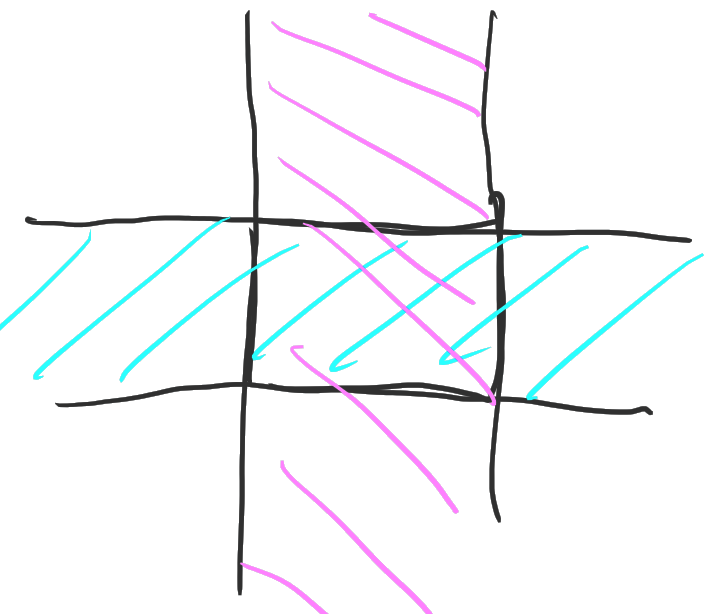
\includegraphics[width=0.25\textwidth]{tapes.png}
            \caption{Двумерные полоски.}
            \label{fig:tapes}
        \end{figure}

        Теперь посмотрим на промежутки:

        \begin{align*}
            I_1=\left[
            \begin{array}{ll}
                (a,\, b) \text{~--- открытое} \Rightarrow\in\FB(\R),\\
                \left[ a,\, b\right)=\bigcap\limits_{n=1}^{\infty} 
                \left(a-\dfrac{1}{n},\, b\right)\Rightarrow \in\FB(\R),\\ 
                \left( a,\, b\right]\text{~--- аналогично}\in\FB(\R),\\
                \left[a,\, b\right]\text{~--- дополнение к открытому}\Rightarrow\in\FB(\R).
            \end{array}
            \right .
        \end{align*}

        Аналогично множества $(I_1\times\R\times\ldots\times\R),\,
        (\R\times I_2\times\ldots\times \R),\,\ldots,\,
        (\R\times\R\times\ldots\times I_d)\in\FB(\R^d)$. А следовательно и их пересечение является
        борелевским множеством. 

        Итак, доказано, что $K_d\subset \FB(\R^d)\Rightarrow \sigma(K_d)\subset\FB(\R^d)$.

        Докажем теперь, что $\FB(\R^d)\subset \sigma(K_d)$. Так как 
        $\FB(\R^d)=\sigma(\tau)$ (см. определение), то достаточно доказать, что 
        $\tau\subset \sigma(K_d)$, в самом деле, если $\tau\subset \sigma(K_d)$, то 
        $\sigma(\tau)\subset \sigma(K_d)$ в силу минимальности $\sigma(\tau)$ по вложению.

        Пусть $U\in\tau$. Докажем, что $U\in\sigma(K_d)$.

        \begin{figure}[!ht]
            \centering
            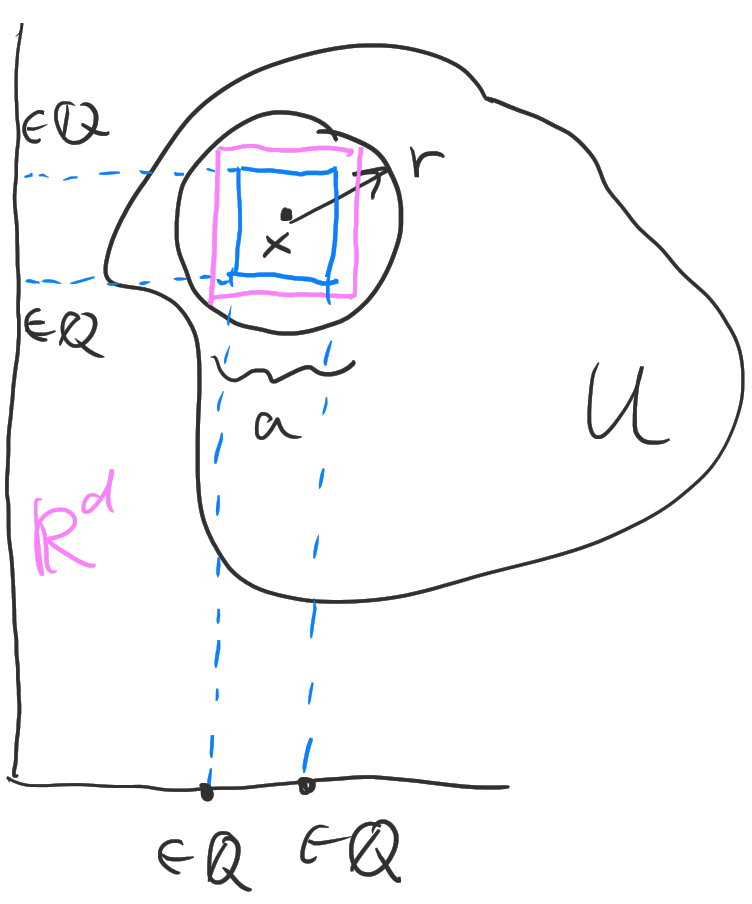
\includegraphics[width=0.6\textwidth]{upic.png}
            \caption{Множество $U$.}
            \label{fig:upic}
        \end{figure}

        $U$ открытое, поэтому $\forall x\in U\ \exists r>0:\ B_r(x)\subset U$, где $B_r(x)$~--- 
        $d$"=мерный шар радиуса $r$ с центром в точке $x$. Поймем какого размера должен быть 
        $d$"=мерный куб, чтобы его можно было вписать в данный шар. Должно выполнится следующее 
        неравенство: $\left(\dfrac{a}{2}\right)^2\cdot d\leqslant r^2$, где $a$~--- искомая сторона
        куба (неравенство следует из теоремы Пифагора: полудиагональ куба складывается из $d$ частей, 
        каждая длиной $\frac{a}{2}$). Откуда $a\leqslant \dfrac{2r}{\sqrt{d}}$. Таким образов любое 
        открытое множество можно представить в виде объединения таких кубиков (на рисунке \ref{fig:upic} это розовый квадрат),
        а кубики уже принадлежат семейству клеточных множеств.
        
        Но возникает проблема: такое объеденение кубиков может оказаться более чем счётным, поэтому сделаем финт ушами:
        сожмём кубик так, чтобы координаты его граней были рациональными (на рисунке это синий квадратик) и обзовем его $Q_x$.
        Множество таких кубов счётно, так как все такие кубы можно параметризовать точками $\Q^{2d}\Rightarrow$ данное семейство 
        счётно. 

        Тогда $\forall x\in U$ поставим в соответствие соответствующий куб $Q_x\subset B_r(x)\subset U$ и 
        $U=\bigcup\limits_{x\in U}\{x\}\subset \bigcup\limits_{x\in U}Q_x$~--- представимо в виде 
        не более чем счётного объединения, так как число кубов счётно и значит $U=\bigcup\limits_{x\in U}Q_x\in\sigma(K_d)$.

    \end{proof} 
\end{claim}

\subsection{Теорема Дынкина.}

\begin{definition}
    Семейство $\F\subset \CP(X)$ называется:
    \begin{enumerate}[label=\arabic*)]
        \item \mdef{$\pi$"=системой}, если $\forall A,\, B\in\F$ выполнено, что $A\cap B\in\F$;
        \item \mdef{$\lambda$"=системой}, если, во-первых, $\varnothing\in\F$, во-вторых,
        $\forall A\in\F$ выполнено, что $A^C\in\F$, а также для любых попарно непересекающихся 
        $D_1,\, \ldots,\, D_n,\,\ldots\in\F$ выполнено $\bigsqcup\limits_{k=1}^{\infty} D_k\in\F$.
    \end{enumerate}
\end{definition}

\begin{exercise}
    $\lambda$"=система в общем случае не всегда является $\pi$"=системой. Например, пусть 
    $X=\{1,\,2,\,3,\,4\}$ и 
    \[
        \F = \{\varnothing,\, X,\, \{1,\,2\},\, \{1,\,3\},\,\{1,\,4\},\,\{2,\,3\},\,\{2,\,4\},\,\{3,\,4\}\}.    
    \]
    Легко видеть, что это $\lambda$"=система, но не $\pi$"=система, так как $\F$ не замкнута относительно пересечения.
\end{exercise}

На прошлой лекции было доказано следующее утверждение (теперь в новой терминологии):
\begin{claim}
    $\F\subset\CP(X)$ является $\sigma$"=алгеброй тогда и только тогда, когда $\F$ 
    одновременно является $\pi$"=системой и $\lambda$"=системой.
\end{claim}

\begin{figure}[!ht]
    \centering
    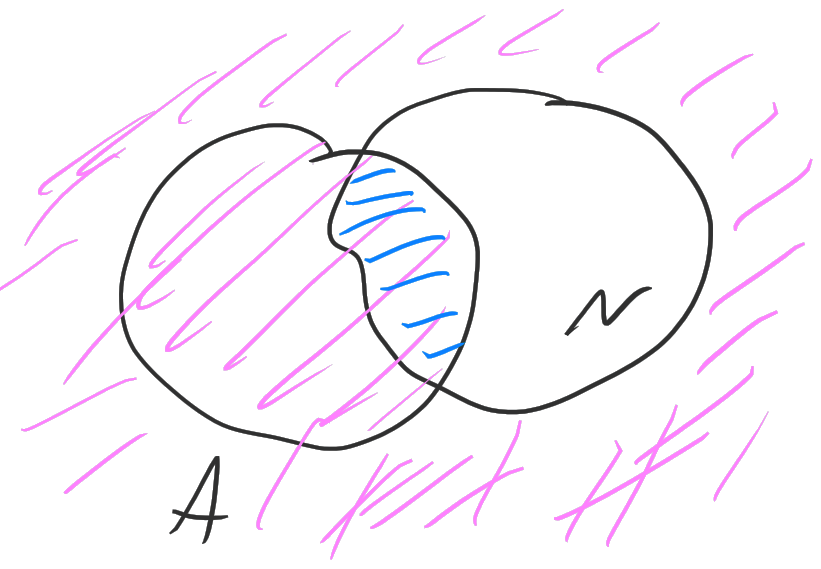
\includegraphics[width=0.5\textwidth]{sets.png}
    \caption{К теореме Дынкина (\ref{theorem:dynkin})}
    \label{fig:sets}
\end{figure}

\begin{theorem}[Дынкин]
    \label{theorem:dynkin}

    Пусть $\F\subset\CP(X)$~--- $\pi$"=система, $\CE\subset\CP(X)$~--- $\lambda$"=система и
    $\F\subset\CE$. Тогда $\sigma(\F)\subset\CE$ (равенство возможно).

    \begin{proof}
        Пусть $\CD\subset \CP(X)$~--- пересечение всех $\lambda$"=систем $\CG\subset\CP(X)$, 
        таких что $\F\subset\CG$. Докажем, что $\sigma(\F)\subset\CD$, для этого достаточно доказать, 
        что $\CD$ является $\sigma$"=алгеброй (снова в силу минимальности).

        Заметим, что $\CD$~--- $\lambda$"=система (доказывается так же как и факт о том, что пересечение сигма-алгебр является
        сигма-алгеброй). Тогда достаточно показать, что $\CD$~--- $\pi$"=система, то есть, что 
        $\forall M,\, N\in\CD$ выполняется, что $M\cap N\in\CD$.

        Введем обозначение: $\CH(M)=\{N\in\CD:\: M\cap N\in\CD\}$, где $M$~--- любой элемент $\CD$. То есть 
        условие о замкнутости по пересечению можно переформулировать так: $\forall M\in\CD$ выполнено $\CH(M)=\CD$.

        \begin{lemma}
            $\forall M\in\CD$ верно, что $\CH(M)$ является $\lambda$"=системой.

            \begin{proof}
                Во-первых, $\varnothing\in\CH(M)$, так как $\forall N\in\CD:\ \varnothing\cap N=\varnothing\in\CD$ по определению.

                Во-вторых, докажем, что $\CH(M)$ замкнуто относительно взятия дополнений. Пусть $A\in\CH(M)$. 
                Заметим, что
                \begin{equation}
                    \label{eq:lemmastate}
                    A\in\CH(M)\ \forall M\in\CD\Leftrightarrow\forall N\in\CD:\ A\cap N\in\CD.
                \end{equation}
                И в частности 
                \[
                    A^C\in\CH(M)\ \forall M\in\CD\Leftrightarrow\forall N\in\CD:\ A^C\cap N\in\CD.    
                \]
                Правое условие, в силу того, что $\CD$~--- $\lambda$"=система эквивалентно тому, что 
                $(A^C\cap N)^C\in\CD$ (из замкнутости по дополнению). Но $(A^C\cap N)^C=A\cup N^C=(A\cap N)\sqcup N^C\in\CD$ 
                (см. рис. \ref{fig:sets}). Итак, $A^C\in\CH(M)$.

                Докажем замкнутость относительно дизъюнктных объединений. Пусть 
                $A_1,\,\ldots,\,A_n,\,\ldots\in\CH(M)$ попарно не пересекаются. Тогда $\forall N\in\CD$:
                \[
                    \left(\bigsqcup_{n=1}^{\infty}A_n\right)\cap N=\bigsqcup_{n=1}^{\infty}\left(A_n\cap N\right)\in \CD,
                \]
                так как $A_n\cap N\in\CD$ (см. условие \eqref{eq:lemmastate}) и $\CD$~--- $\lambda$"=система.

            \end{proof}
        \end{lemma}

        Пусть $M\in\F\subset\CD$ (по построению). Зададимся вопросом: для каких $N\in\CD$ выполнено, что $M\cap N\in\CD$?
        Если $N\in\F$, то $M\cap N\in\F$, так как $\F$~--- $\pi$"=система. Поэтому $\forall N\in\F$
        выполнено $N\in\CH(M)$, то есть $\F\subset\CH(M)$, а значит $\CH(M)$~--- одна из $\lambda$"=систем, включающих в себя 
        $\F$, следовательно, в силу минимальности по вложению, $\CD\subset\CH(M)$ для $\forall M\in\F$, 
        то есть $\forall N\in\CD,\, \forall M\in\F$ выполнено $M\cap N\in\CD$. А значит $\forall N\in\CD$ выполнено $\F\subset\CH(N)$, и 
        снова в силу минимальности $\CD\subset \CH(N)$. Итак, $\forall N,\, M\in\CD$ выполнено $M\cap N\in\CD$.
        
    \end{proof}
\end{theorem}


\begin{task}{4}
	Рассмотрим функцию $\nu: \CP(\R) \rightarrow [0, +\infty]$ вида 
	$$
	\nu(A) = \#\{k \in \Z: [k, k+1)\cap A \neq \varnothing\},~ A \subset \R
	$$ 
где $\#B = n$ если множество $B$ состоит из $n \in \N_0$ элементов и $\#B = +\infty$ если множество $B$ бесконечно. Докажите, что $\nu$ является внешней мерой. Опишите все $\nu$-аддитивные множества.
\end{task}

\begin{solution}
	\begin{itemize}
		\item Докажем, что $\nu$ --- счетно-аддитивна:
		\begin{align*}
			\nu\left(\bigcup_{k=1}^{\infty} A_k\right) &= \#\left\{k \in \Z \mid 
			[k,k+1) \cap \bigcup_{k=1}^{\infty}A_k \neq \varnothing\right\} \leq \\ 
			&\leq \#\left\{\bigcup_{k=1}^{\infty}\left\{k\in \Z \mid 
			[k,k+1)\cap A_k \neq \varnothing \right\}\right\} = \sum_{k=1}^{\infty}\nu(A_k)
		\end{align*}
	
		\item 
		Докажем, что $\nu$-аддитивные множества это 
		$$
		A_\nu = \left\{\bigcup_{k=1}^{\infty}I_k\mid I_k \text{--- промежуток с целыми концами}\right\}
		$$
		Пусть $A \in A_\nu$, докажем, что 
		$$
		\nu(T) = \nu(T \cap A ) + \nu(T \cap A^c)
		$$
		\begin{equation}\label{task_4_f1}
		\nu(T\cap A) = \#\left\{k \in \Z \mid [k,k+1)\cap A\cap T \neq \varnothing \right\} = \#\left\{k \in \Z \mid ([k,k+1) \cap T)\cap A \right\}
		\end{equation}
		С другой стороны:
		\begin{equation}\label{task_4_f2}
		\nu(T\cap A^c) = \#\left\{k \in \Z \mid [k,k+1)\cap A^c\cap T \neq \varnothing \right\} = \#\left\{k \in \Z \mid ([k,k+1) \cap T)\cap A^c \right\}
		\end{equation}
		В силу того, $A$ и $A^c$ состоит из промежутков с целыми концами, то из \ref{task_4_f1}, \ref{task_4_f2}:
		$$
		\nu(T \cap A) + \nu(T \cap A^c) = \#\left\{k\in \Z \mid [k,k+1) \cap T \neq \varnothing \right\} = \nu(T)
		$$
		Пусть в $A_\nu$ есть множество $A$, точка границы замыкания которого --- не целая. 
		Тогда рассмотрим часть этого множества $A' \subset A$ без всех остальных укладывающихся в это множество
		единичных промежутков, $A' \in A_\nu$, так как $A_\nu$ --- сигма-алгебра. Не умаляя общности считаем, что 
		$$
		A' = [k,x), ~ x\notin \Z,~ x < k+1
		$$
		(случай отрезка рассматривается аналогично), тогда для $T = [k,k+1]$:
		$$
		1 = \nu(T) = \nu(T\cap A) + \nu(T \cap A^c) = 1 + 1 =2
		$$
		Таким образом $A_\nu$ действительно все $\nu$-аддитивные множества.
		\end{itemize}
	
	
\end{solution}



% \newpage
\section{Additional information}
\end{document}